\documentclass[border=10pt]{standalone}

\usepackage{tikz}
\usepackage{tikzsymbols}
\usetikzlibrary{calc,patterns,shapes.geometric}

\def\centerarc[#1](#2)(#3:#4:#5){\draw[#1] ($(#2)+({#5*cos(#3)},{#5*sin(#3)})$) arc (#3:#4:#5);}

\begin{document}
	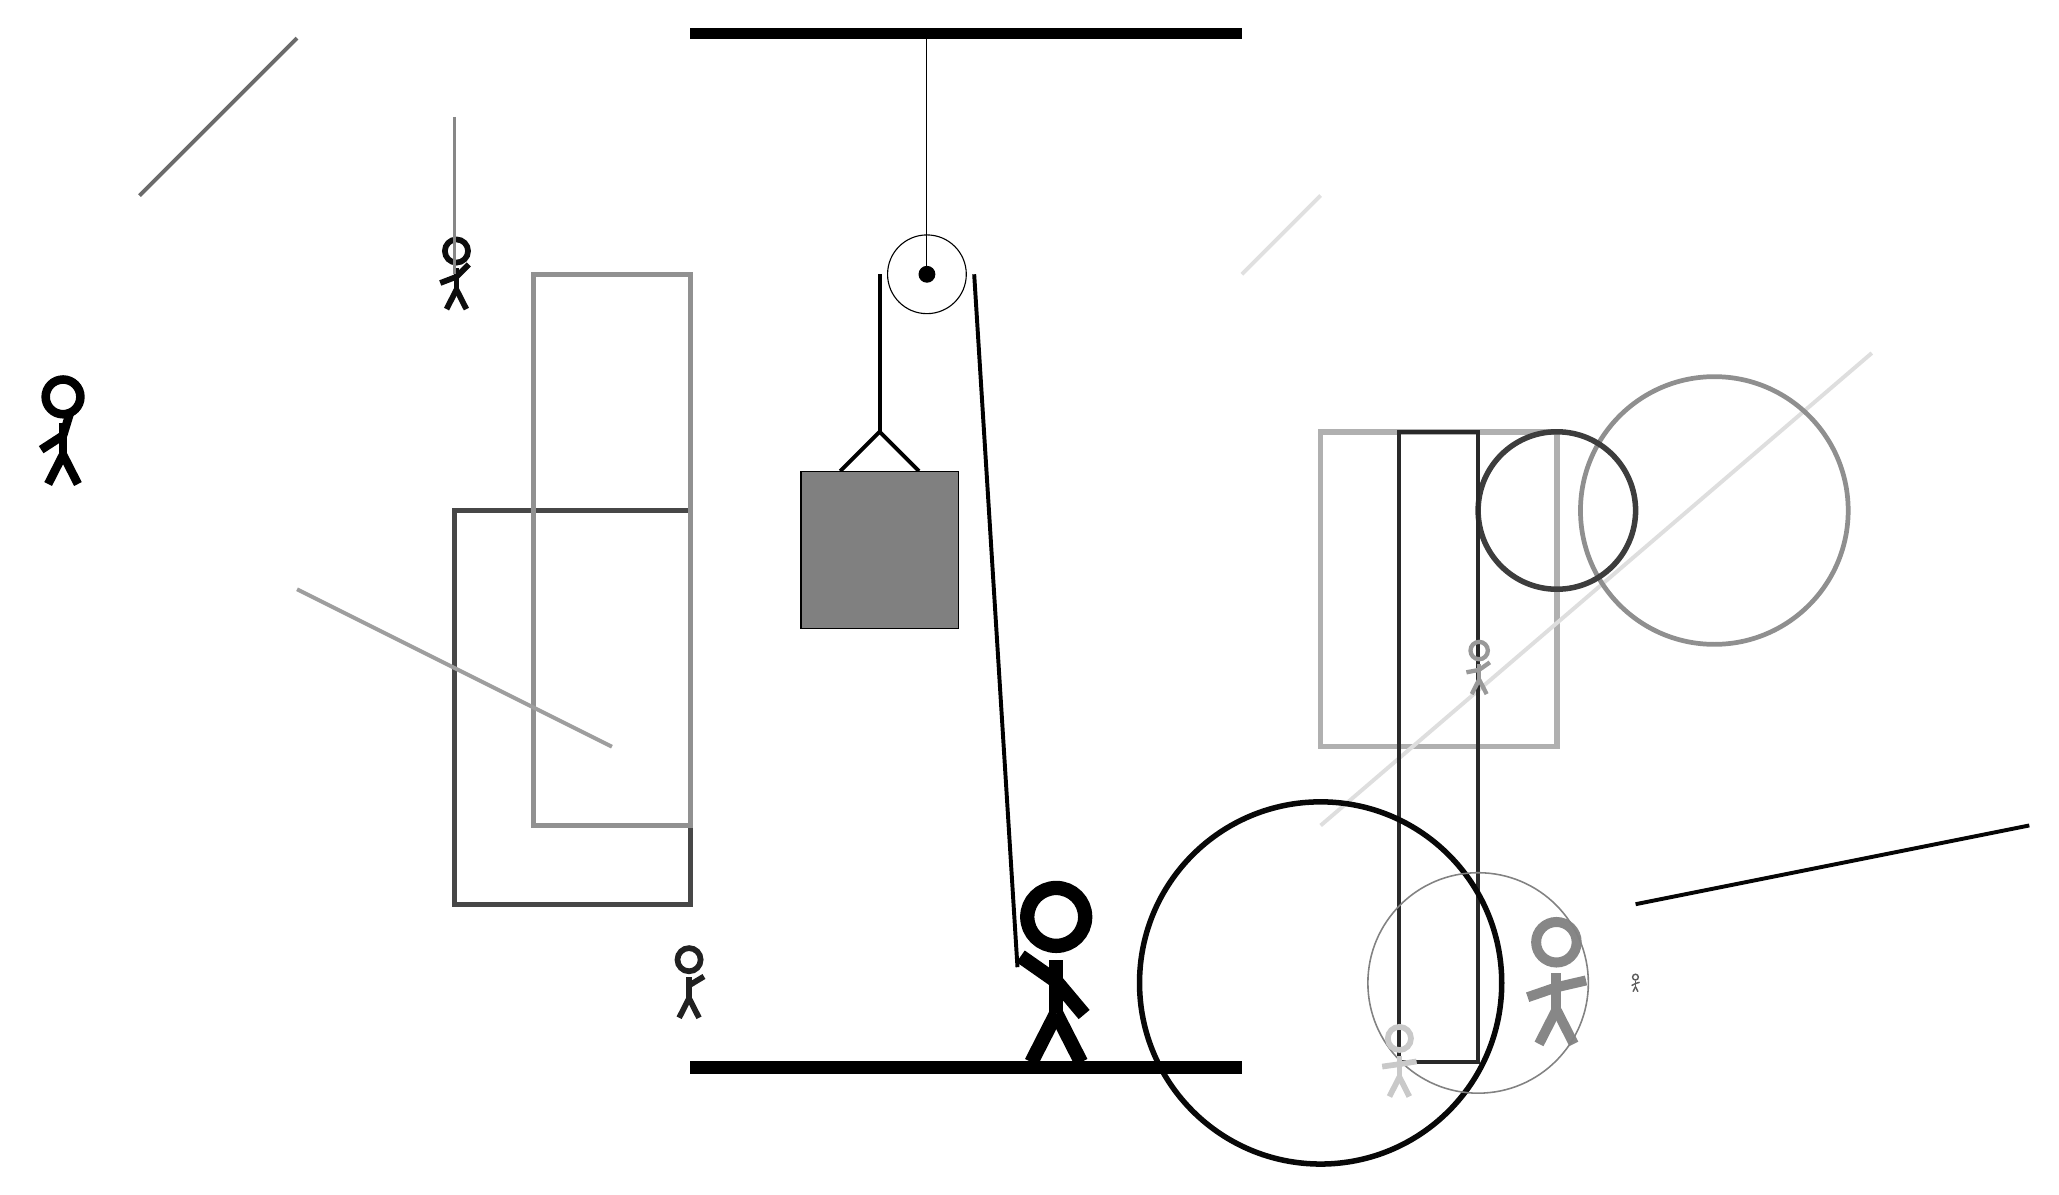
\begin{tikzpicture}
		%%%%% START %%%%%
		
		\draw[fill=black] (-2, 10) rectangle (5, 10.125);
		
		\draw (1, 7) circle (0.5);
		\draw[fill=black] (1, 7) circle (0.1);
		\draw (1, 10) -- (1, 7);
		
		\draw[line width=0.5mm] (-0.1, 4.5) -- (0.4, 5.0) -- (0.9, 4.5);
		\draw[fill=black!50] (-0.6, 4.5) rectangle (1.4, 2.5);
		
		\draw[line width=0.7mm, color=black!31] (6, 1) rectangle (9, 5);
		
		\draw[line width=0.6mm, color=black!72] (-2, 4) rectangle (-5, -1);
		\node[line width=0.4mm, color=black!47] at (9, -2) {\Strichmaxerl[7][19][13]};
		\draw[line width=0.6mm, color=black!43] (-2, 0) rectangle (-4, 7);
		\node[line width=0.5mm, color=black!63] at (10, -2) {\Strichmaxerl[1][27][18]};
		
		\node[line width=0.2mm, color=black!87] at (-2, -2) {\Strichmaxerl[4][90][31]};
		
		\draw[line width=0.5mm, color=black!13](6, 0) -- (13, 6);
		
		\draw [line width=0.6mm, color=black!44](11, 4) circle (1.7);
		\draw[line width=0.5mm, color=black!98](10, -1) -- (15, 0);
		
		\node[line width=0.4mm, color=black!100] at (-10, 5) {\Strichmaxerl[6][33][73]};
		\node[line width=0.6mm, color=black!95] at (-5, 7) {\Strichmaxerl[4][21][45]};
		\draw[line width=0.5mm, color=black!12](6, 8) -- (5, 7);
		\draw[line width=0.5mm, color=black!38](-7, 3) -- (-3, 1);
		
		\draw [line width=0.7mm, color=black!76](9, 4) circle (1.0);
		\draw[line width=0.5mm, color=black!84] (7, -3) rectangle (8, 5);
		\node[line width=0.3mm, color=black!40] at (8, 2) {\Strichmaxerl[3][11][35]};
		\draw [line width=0.6mm, color=black!36](7, 7) circle (0.0);
		\draw [line width=0.7mm, color=black!97](6, -2) circle (2.3);
		\draw[line width=0.5mm, color=black!47](-5, 9) -- (-5, 7);
		\draw[line width=0.5mm, color=black!58](-7, 10) -- (-9, 8);
		\draw [line width=0.2mm, color=black!49](8, -2) circle (1.4);
		\node[line width=0.5mm, color=black!21] at (7, -3) {\Strichmaxerl[4][8][9]};
		
		
		\draw[line width=0.5mm] (0.4, 7) -- (0.4, 5.0);
		\centerarc[line width=0.5mm](1, 7)(0:180:0.6);
		\draw[line width=0.5mm](1.6, 7) -- (2.15, -1.8);
		
		\node at (2.6, -1.9) {\Strichmaxerl[10][-35][-50]};
		
		\draw[fill=black] (-2, -3) rectangle (5, -3.15);
		
		%%%%% END %%%%%
	\end{tikzpicture}
\end{document}